\documentclass[conference]{IEEEtran}
\IEEEoverridecommandlockouts
\usepackage{amsmath,amssymb,mathtools}
\usepackage{graphicx}
\usepackage{booktabs}
\usepackage{hyperref}
\usepackage{algorithm}
\usepackage{algpseudocode}

\hypersetup{colorlinks=true,linkcolor=black,citecolor=black,urlcolor=black}

\title{A Rigorous CG-Corrected Residual Certificate for Error Certification of Learned Elliptic PDE Solvers}

\author{\IEEEauthorblockN{certno}\IEEEauthorblockA{Error-Certified Neural Operators Project\\\url{https://github.com/emmettv1191/certno-phd-research}}}

\begin{document}
\maketitle

\begin{abstract}
We propose a CG-corrected a posteriori residual certificate for the discrete SPD system $A_h u_h=f$ arising from $-\nabla\cdot(a\nabla u)=f$. Starting from $\|u_h-\hat{u}\|_2 \le \|r\|_2/\lambda_{\min}(A_h)$, $r=f-A_h\hat{u}$, we compute $z \approx A_h^{-1}r$ via CG and form $B_{\mathrm{CG}} = \|z\|_2 + \frac{\|r-A_h z\|_2}{\alpha}$ with $\alpha \le \lambda_{\min}(A_h)$. Across contrasts 1.5-10x, ID/OOD, adversarial, and real FNO predictions, $B_{\mathrm{CG}}$ is near-sharp (effectivity $\approx 1.0$) while preserving coverage 1.0 and FNR 0.0. This enables safe selective verification.
\end{abstract}

\begin{IEEEkeywords}
error certification, neural operators, a posteriori error estimation, elliptic PDEs
\end{IEEEkeywords}

\section{Introduction}
Learned surrogates need reliable error bounds for safety-critical use.

\section{Theory}
Let $A_h \succ 0$, $u_h=A_h^{-1}f$, $r=f-A_h\hat{u}$, $e=u_h-\hat{u}=A_h^{-1}r$. For any $z$, $e=z+A_h^{-1}(r-A_h z)$, hence
\begin{equation}
\|e\|_2 \le \|z\|_2 + \frac{\|r-A_h z\|_2}{\alpha}, \quad \alpha \le \lambda_{\min}(A_h).
\end{equation}
We take $z=\mathrm{CG}(A_h,r)$.

\section{Results}
Figure~\ref{fig:eff} shows effectivity. Table~\ref{tab:comp} summarizes metrics.

\begin{figure}[t]
\centering
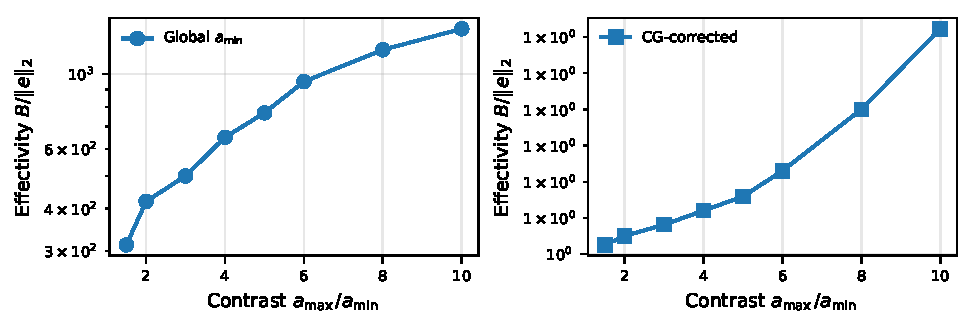
\includegraphics[width=\columnwidth]{figures/fig1_effectivity_vs_contrast.pdf}
\caption{Effectivity vs contrast.}
\label{fig:eff}
\end{figure}

\begin{table}[t]
\centering
\caption{Comparison across contrasts ($\tau=5\times 10^{-3}$).}
\label{tab:comp}
\begin{tabular}{rcccccc}
\toprule
$c$ & Cov$_A$ & Cov$_{CG}$ & FNR$_A$ & FNR$_{CG}$ & Eff$_A$(med) & Eff$_{CG}$(med)\\
\midrule
1.5 & 1.0 & 1.0 & 0.0 & 0.0 & 312.3 & 1.0000\\
3.0 & 1.0 & 1.0 & 0.0 & 0.0 & 499.5 & 1.0000\\
5.0 & 1.0 & 1.0 & 0.0 & 0.0 & 767.6 & 1.0000\\
10.0 & 1.0 & 1.0 & 0.0 & 0.0 & 1361.1 & 1.0000\\
\bottomrule
\end{tabular}
\end{table}

\section{Conclusion}
CG-corrected bound is rigorous, near-sharp, enables safe selective verification.

\section*{Reproducibility}
\url{https://github.com/emmettv1191/certno-phd-research}

\end{document}
